\documentclass[border=12pt]{standalone}
\def\pgfsysdriver{pgfsys-dvisvgm.def}
\usepackage[dvisvgm]{xcolor}
\usepackage{xeCJK}
\setCJKmainfont{HaranoAjiGothic-Regular.otf}[BoldFont=HaranoAjiGothic-Bold.otf]
\setCJKsansfont{HaranoAjiGothic-Regular.otf}[BoldFont=HaranoAjiGothic-Bold.otf]
\usepackage{amsmath,amssymb,tikz,lmodern}
\usetikzlibrary{arrows.meta,calc}
\renewcommand{\familydefault}{\sfdefault}
\hyphenpenalty=10000
\exhyphenpenalty=10000
\definecolor{ink}{HTML}{25322F}
\definecolor{green}{HTML}{246657}
\definecolor{tint}{HTML}{EEF4F0}
\definecolor{soft}{HTML}{C6D2CC}
\definecolor{muted}{HTML}{52615B}
\definecolor{tool}{HTML}{875832}
\newif\ifJapanese
\newcommand{\Tx}[2]{\ifJapanese #1\else #2\fi}
\newcommand{\Link}[2]{\special{dvisvgm:raw <a xlink:href="#1">}{\setlength{\fboxsep}{0pt}\colorbox{white}{\color{green}\underline{\strut #2}}}\special{dvisvgm:raw </a>}}
\newcommand{\Paper}[2]{\Link{\csname paper#1\endcsname}{#2}}
\newcommand{\Input}[2]{\Link{\catalogbase\string##connection-#1}{#2}}
\newcommand{\Head}[2]{{\color{green}\bfseries\Tx{#1}{#2}}\\[5pt]}
\tikzset{
 card/.style={draw=soft,fill=white,rounded corners=2pt,align=left,text=ink,font=\fontsize{11}{15}\selectfont,inner xsep=11pt,inner ysep=10pt,text width=6cm,minimum height=2.4cm},
 result/.style={card,draw=green,fill=tint,line width=.8pt},
 reason/.style={align=left,text=muted,font=\fontsize{10}{13}\selectfont,inner sep=0pt,text width=5.2cm},
 edge/.style={-{Stealth[length=2.4mm]},draw=green,line width=1pt},
 auxiliary/.style={edge,draw=tool,dashed},
 premise/.style={edge,densely dotted,line width=1.5pt},
}
% Vertical arrows and explanations occupy separate gutters.
\newcommand{\Flow}[4]{
 \coordinate (#2start) at ($(#1.south)+(-2.85,0)$);
 \coordinate (#2end) at ($(#2.north)+(-2.85,0)$);
 \draw[#3] (#2start)--(#2end);
 \node[reason,anchor=west] at ($(#2start)!.5!(#2end)+(.55,0)$) {#4};
}

\Japanesefalse
\newcommand{\catalogbase}{/OpenAI-Math-Digest/en/catalog/034/}
\expandafter\def\csname paperlog-abundance-characteristic-zero\endcsname{/OpenAI-Math-Digest/en/papers/log-abundance-characteristic-zero/\string##induction}
\expandafter\def\csname paperschnell-fiber-spaces\endcsname{/OpenAI-Math-Digest/en/papers/schnell-fiber-spaces/\string##argument}
\expandafter\def\csname paperminimal-metrics-injectivity\endcsname{/OpenAI-Math-Digest/en/papers/minimal-metrics-injectivity/\string##proof-1}
\expandafter\def\csname paperfourfold-nonvanishing\endcsname{/OpenAI-Math-Digest/en/papers/fourfold-nonvanishing/\string##proof-1}
\expandafter\def\csname paperlifting-adjoint-sections\endcsname{/OpenAI-Math-Digest/en/papers/lifting-adjoint-sections/\string##proof-1}
\expandafter\def\csname paperrelative-denominators\endcsname{/OpenAI-Math-Digest/en/papers/relative-denominators/\string##proof-1}
\expandafter\def\csname paperarithmetic-stein-degree\endcsname{/OpenAI-Math-Digest/en/papers/arithmetic-stein-degree/\string##proof-1}
\expandafter\def\csname papereffective-log-iitaka-fourfolds\endcsname{/OpenAI-Math-Digest/en/papers/effective-log-iitaka-fourfolds/\string##proof-1}
\expandafter\def\csname paperuniform-pluricanonical-iitaka\endcsname{/OpenAI-Math-Digest/en/papers/uniform-pluricanonical-iitaka/\string##proof-1}
\expandafter\def\csname paperuniform-log-iitaka\endcsname{/OpenAI-Math-Digest/en/papers/uniform-log-iitaka/\string##proof-1}
\expandafter\def\csname paperuniform-slc-indices\endcsname{/OpenAI-Math-Digest/en/papers/uniform-slc-indices/\string##proof-1}
\expandafter\def\csname paperabundance-after-nonvanishing\endcsname{/OpenAI-Math-Digest/en/papers/abundance-after-nonvanishing/\string##proof-1}
\expandafter\def\csname paperconditional-kahler-fourfolds\endcsname{/OpenAI-Math-Digest/en/papers/conditional-kahler-fourfolds/\string##proof-1}
\expandafter\def\csname paperkahler-log-abundance\endcsname{/OpenAI-Math-Digest/en/papers/kahler-log-abundance/\string##proof-1}
\begin{document}
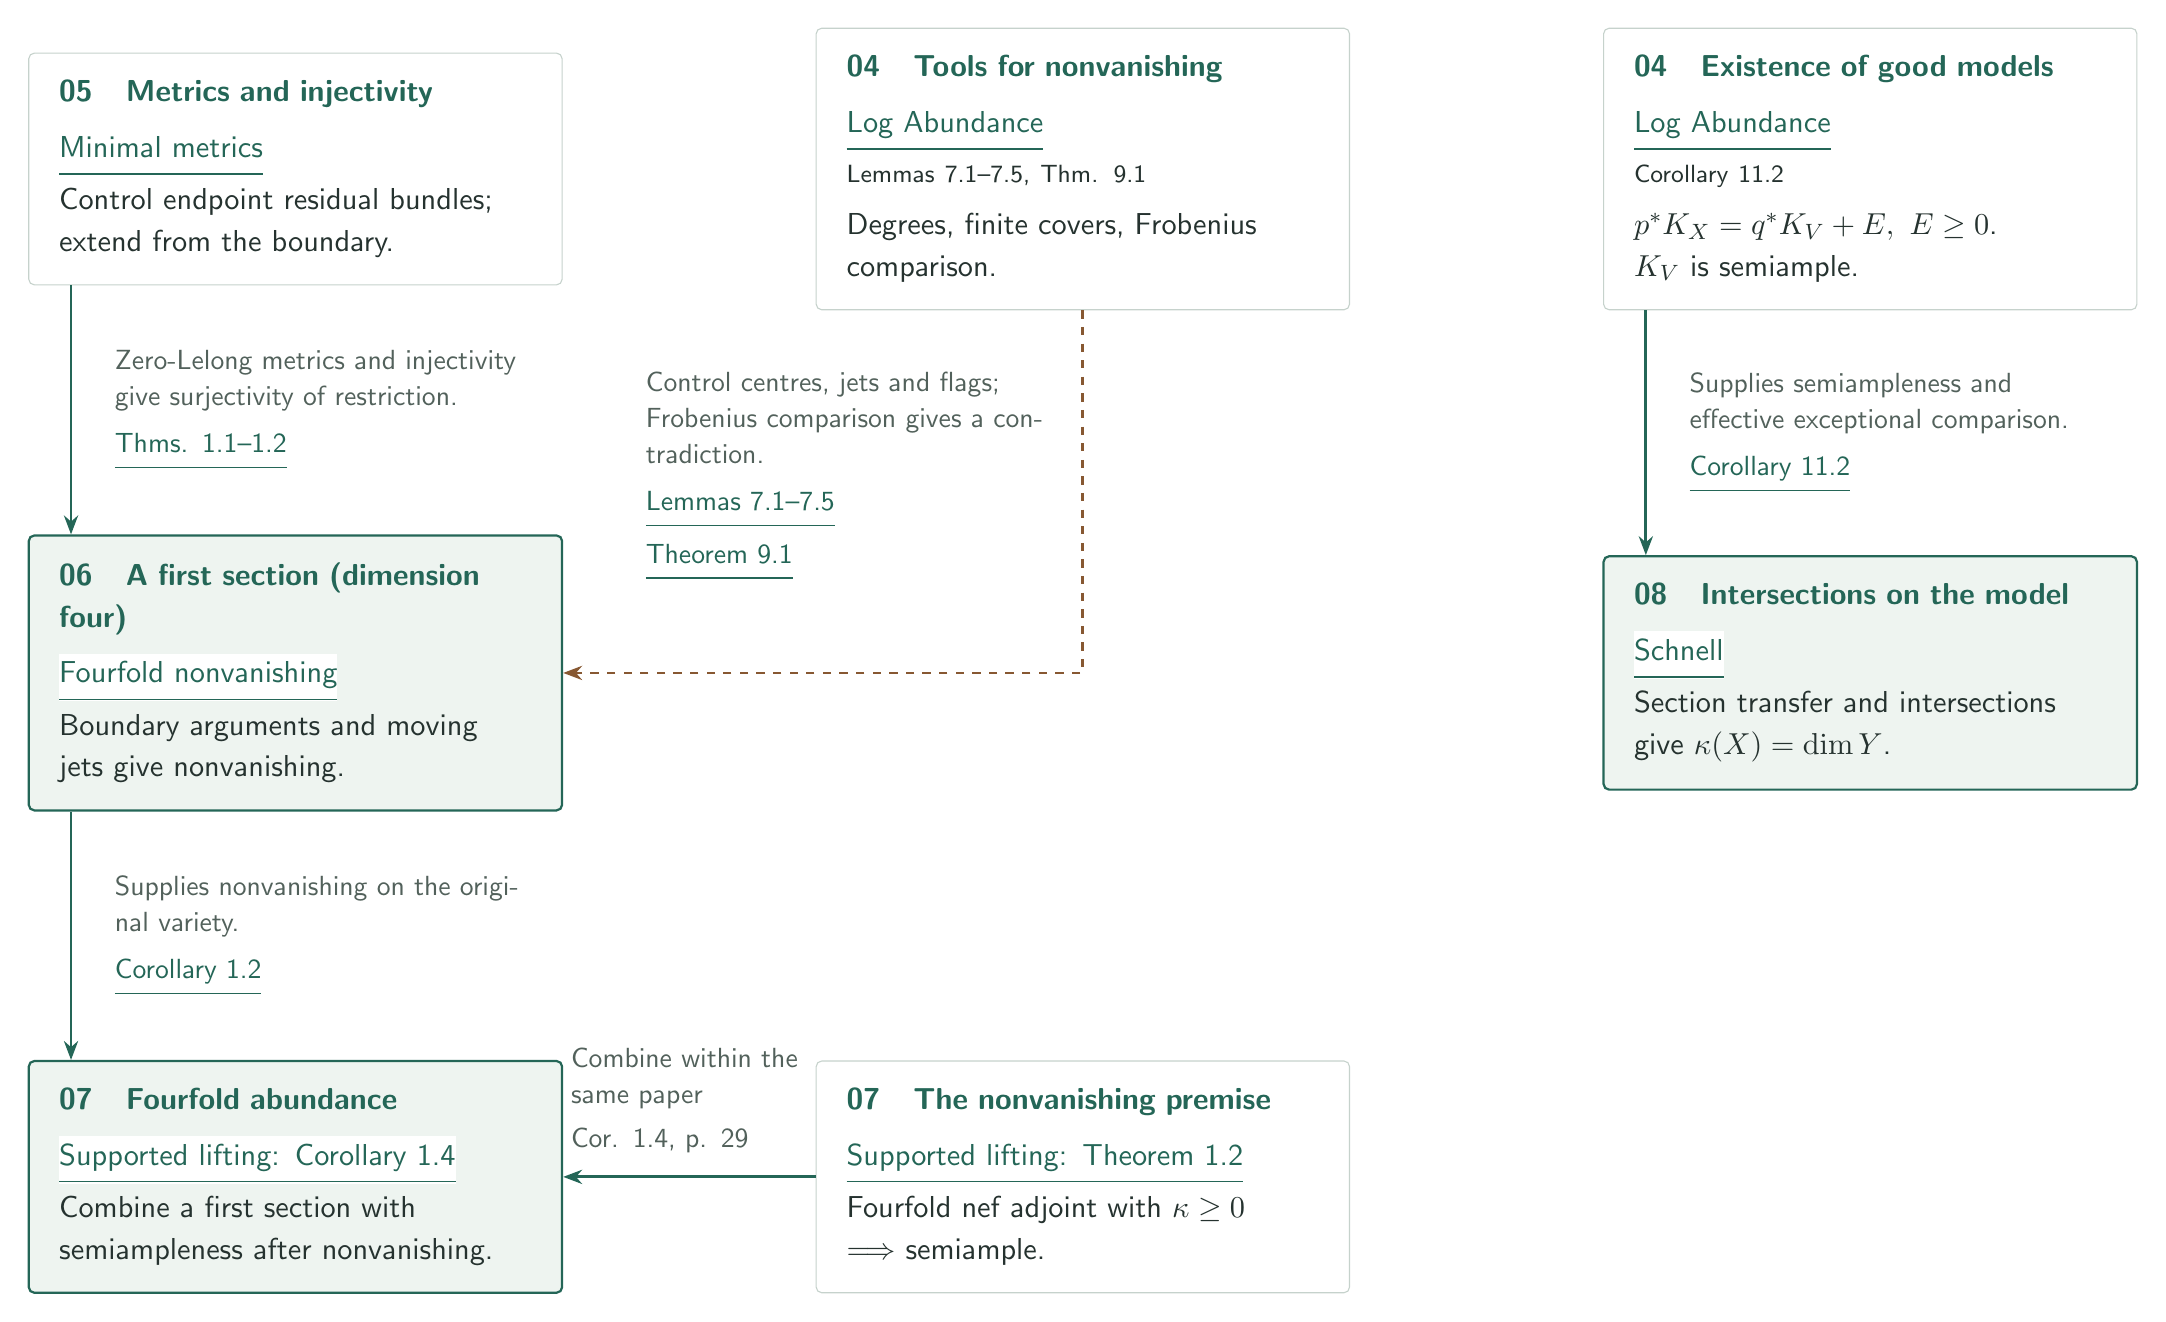
\begin{tikzpicture}
\node[card] (metrics) at (0,0) {\Head{05\quad 計量と内部単射性}{05\quad Metrics and injectivity}
\Paper{minimal-metrics-injectivity}{Minimal metrics}\\[4pt]
\Tx{端点の残余束を扱い、境界から延長する。}{Control endpoint residual bundles; extend from the boundary.}};
\node[card] (tools) at (10,0) {\Head{04\quad 非消滅のための道具}{04\quad Tools for nonvanishing}
\Paper{log-abundance-characteristic-zero}{Log Abundance}\\[3pt]{\small Lemmas 7.1--7.5, Thm. 9.1}\\[4pt]
\Tx{次数・有限被覆・Frobenius比較。}{Degrees, finite covers, Frobenius comparison.}};
\node[card] (models) at (20,0) {\Head{04\quad 良いモデルの存在}{04\quad Existence of good models}
\Paper{log-abundance-characteristic-zero}{Log Abundance}\\[3pt]{\small Corollary 11.2}\\[4pt]
$p^*K_X=q^*K_V+E,\ E\ge0$.\\
\Tx{$K_V$ は semiample。}{$K_V$ is semiample.}};
\node[result] (nv) at (0,-6.4) {\Head{06\quad 四次元の最初の切断}{06\quad A first section (dimension four)}
\Paper{fourfold-nonvanishing}{Fourfold nonvanishing}\\[4pt]
\Tx{境界の議論とmoving jetsで非消滅へ。}{Boundary arguments and moving jets give nonvanishing.}};
\Flow{metrics}{nv}{edge}{\Tx{零Lelong計量・内部単射性\\から制限写像の全射性へ。}{Zero-Lelong metrics and injectivity\\give surjectivity of restriction.}\\[4pt]\Input{metrics-nonvanishing}{Thms. 1.1--1.2}}
\draw[auxiliary] (tools.south)--(10,-6.4)--(nv.east);
\node[reason,text width=5.4cm] at (7.15,-3.9) {\Tx{中心・jet・旗を制御し、\\Frobenius比較で矛盾を得る。}{Control centres, jets and flags;\\Frobenius comparison gives a contradiction.}\\[4pt]
\Input{la-nonvanishing-geometry}{Lemmas 7.1--7.5}\\[3pt]\Input{la-nonvanishing-tool}{Theorem 9.1}};
\node[result] (schnell) at (20,-6.4) {\Head{08\quad モデル上の交点数へ}{08\quad Intersections on the model}
\Paper{schnell-fiber-spaces}{Schnell}\\[4pt]
\Tx{切断の移送と混合交点数で\\$\kappa(X)=\dim Y$ を得る。}{Section transfer and intersections\\give $\kappa(X)=\dim Y$.}};
\Flow{models}{schnell}{edge}{\Tx{半豊富な標準因子と\\有効例外因子の比較式を供給。}{Supplies semiampleness and\\effective exceptional comparison.}\\[4pt]\Input{la-schnell}{Corollary 11.2}}
\node[result] (lifting) at (0,-12.8) {\Head{07\quad 四次元の豊富性}{07\quad Fourfold abundance}
\Paper{lifting-adjoint-sections}{Supported lifting: Corollary 1.4}\\[4pt]
\Tx{最初の切断と、非消滅後の\\semiamplenessを合わせる。}{Combine a first section with\\semiampleness after nonvanishing.}};
\Flow{nv}{lifting}{edge}{\Tx{原多様体上で非消滅を供給。}{Supplies nonvanishing on the original variety.}\\[4pt]\Input{nonvanishing-lifting}{Corollary 1.2}}
\node[card] (after) at (10,-12.8) {\Head{07\quad 非消滅を仮定する段階}{07\quad The nonvanishing premise}
\Paper{lifting-adjoint-sections}{Supported lifting: Theorem 1.2}\\[4pt]
\Tx{nefかつ $\kappa\ge0$ の四次元随伴\\$\Longrightarrow$ semiample。}{Fourfold nef adjoint with $\kappa\ge0$\\$\Longrightarrow$ semiample.}};
\draw[edge] (after.west)--(lifting.east);
\node[reason,text width=3cm,anchor=south] at (5,-12.5) {\Tx{同じ論文内で合流}{Combine within the same paper}\\[3pt]\Tx{Cor. 1.4, p. 29}{Cor. 1.4, p. 29}};
\end{tikzpicture}

\end{document}
